\documentclass[11pt, a4paper]{article}

% --- PACKAGES ---
\usepackage[margin=1in]{geometry}
\usepackage{amsmath}
\usepackage{graphicx}
\usepackage{xcolor}
\usepackage{float}
\usepackage{listings}
\usepackage{hyperref}
\hypersetup{colorlinks=true, linkcolor=blue, urlcolor=blue}

% --- CODE LISTING STYLE ---
\definecolor{codegreen}{rgb}{0,0.6,0}
\definecolor{codegray}{rgb}{0.5,0.5,0.5}
\definecolor{codepurple}{rgb}{0.58,0,0.82}
\definecolor{backcolour}{rgb}{0.98,0.98,0.97}
\lstdefinestyle{mystyle}{
    backgroundcolor=\color{backcolour},   
    commentstyle=\color{codegreen},
    keywordstyle=\color{blue},
    numberstyle=\tiny\color{codegray},
    stringstyle=\color{codepurple},
    basicstyle=\ttfamily\footnotesize,
    breakatwhitespace=false,         
    breaklines=true,                 
    captionpos=b,                    
    keepspaces=true,                 
    numbers=left,                    
    numbersep=5pt,                  
    showspaces=false,                
    showstringspaces=false,
    showtabs=false,                  
    tabsize=2,
    breakautoindent=true,
    postbreak=\mbox{\textcolor{red}{$\hookrightarrow$}\space}
}
\lstset{style=mystyle}

% --- DOCUMENT START ---
\begin{document}

% --- TITLE PAGE ---
\begin{titlepage}
    \centering
    \vspace*{\fill}
    {\Huge\bfseries EE200: Signals, Systems and Networks\par}
    \vspace{1.5cm}
    {\Large\bfseries Practical Report 2: Frequency De-mixer\par}
    \vspace{2cm}
    
    \large\emph{Instructor:}\\ Dr. Tushar Sandhan
        
    \vfill
    {\large \texttt{Aarav Aryaman} \\ \texttt{220012}}\par
    \vspace*{1cm}
    {\large \today\par}
\end{titlepage}

\tableofcontents
\newpage

% --- INTRODUCTION ---
\section{Introduction and Problem Interpretation}
The objective of this task is to design and implement a "frequency de-mixer" system for audio restoration. The input signal, contained in \texttt{song\_with\_2piccolo.wav}, is a music track corrupted by the presence of an unwanted instrumental component that disrupts the intended harmony. The primary goal is to \textbf{recover the original song as faithfully as possible} by suppressing this interfering component and to \textbf{export the cleaned version} as a new audio file.

Initial analysis of the audio revealed three distinct components: a low-frequency drum beat, a mid-frequency synthesized singing voice, and a high-frequency piccolo-like melody. After careful consideration, the "unwanted solo instrumental" was interpreted to be the high-pitched piccolo melody. Its piercing, lead-like nature is the primary source of disruption to the song's main harmony, which is carried by the voice and the foundational beat. Therefore, the task was defined as the surgical removal of the piccolo's frequency components.

The process to reach this conclusion was iterative. Initial interpretations of the problem, such as removing all high frequencies with a low-pass filter or all low frequencies with a high-pass filter, were tested and rejected. A low-pass filter successfully removed the piccolo but also unacceptably muffled the vocals. A high-pass filter removed the drum beat but failed to separate the voice from the piccolo. This process of elimination proved that a more precise filtering strategy was required, leading to the final, successful interpretation.

% --- SIGNAL ANALYSIS ---
\section{Signal Analysis}
The first step in designing the filter system was to \textbf{analyze the frequency characteristics of the input} signal. Various analysis tools were employed to precisely \textbf{isolate the frequency regions} occupied by the unwanted piccolo solo.

\begin{itemize}
    \item \textbf{Spectrogram Analysis:} The spectrogram (Figure \ref{fig:spec_orig}) was used to visualize how the frequency content of the signal changes over time. It clearly revealed the piccolo solo as a series of bright, distinct horizontal bands in the upper frequency range (above 1000 Hz), separate from the lower-frequency content of the voice and drums.
    
    \item \textbf{Power Spectral Density (PSD) Analysis:} The PSD plot (Figure \ref{fig:psd}) was then used to get a quantitative view of the total energy at each frequency across the entire track. This plot confirmed the observations from the spectrogram, showing clear "humps" of energy in three primary regions corresponding to the piccolo's fundamental notes and harmonics.
\end{itemize}

Based on this detailed analysis, the frequency regions of the interfering instrument were isolated, and the following bands were targeted for removal: 1000-2000 Hz, 2450-4150 Hz, and 4300-5300 Hz.

\begin{figure}[H]
    \centering
    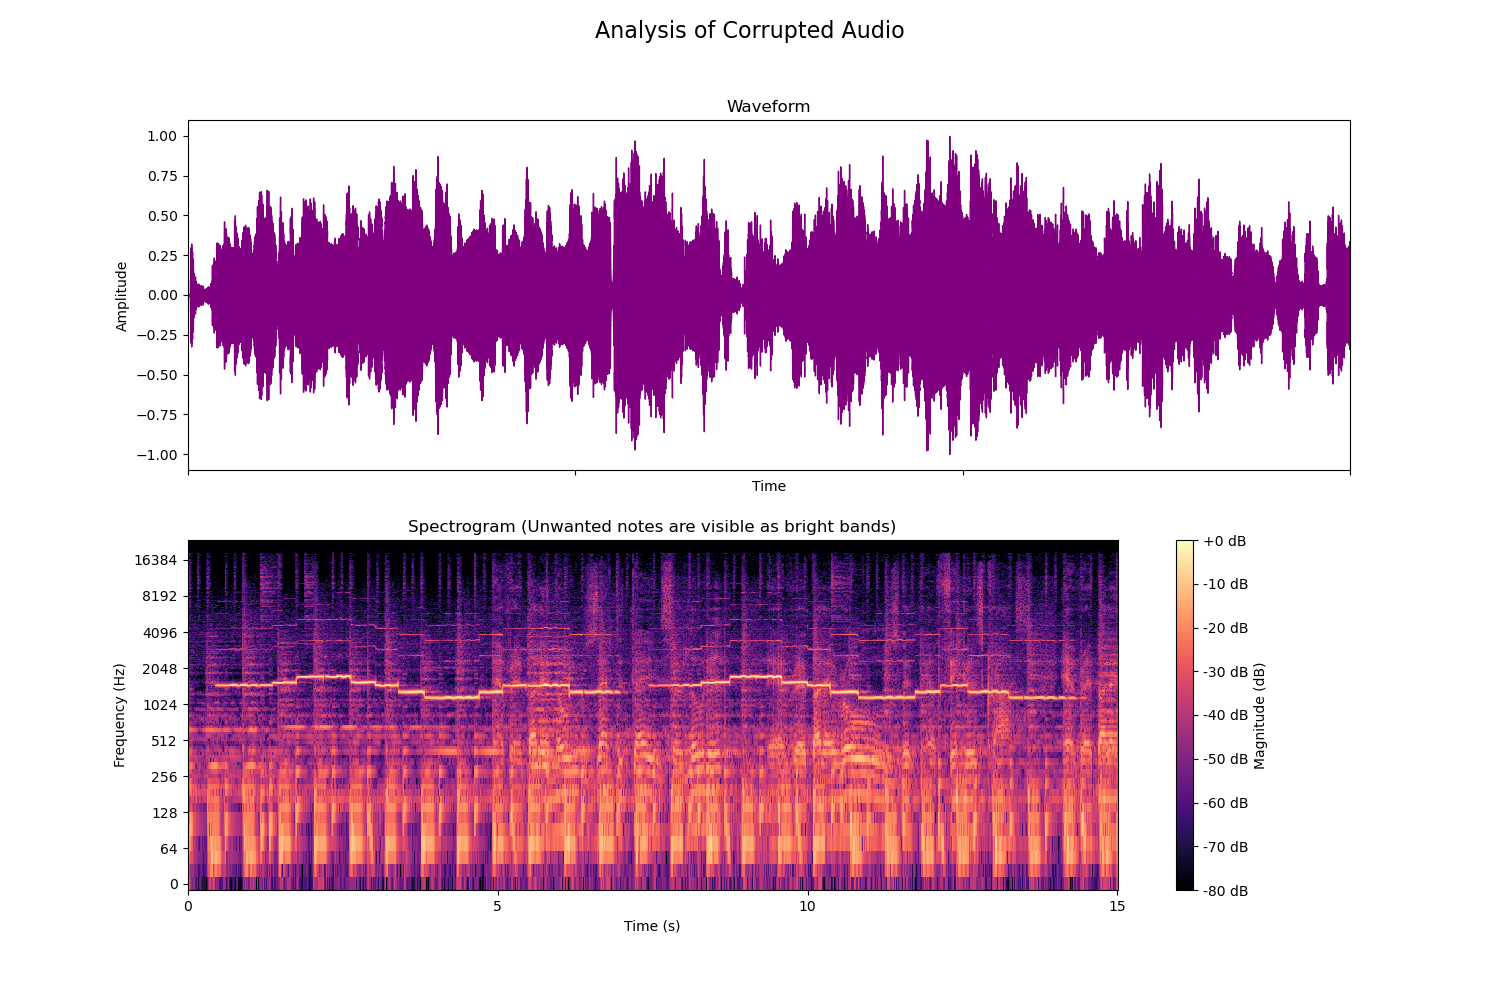
\includegraphics[width=0.9\textwidth]{q2_part1a_corrupted_analysis.png}
    \caption{Spectrogram of the corrupted audio signal. The high-frequency piccolo notes are clearly visible as bright, distinct horizontal bands.}
    \label{fig:spec_orig}
\end{figure}

The spectrogram in Figure \ref{fig:spec_orig} clearly shows the frequency separation between the audio components. The voice and drums occupy the lower part of the spectrum, while the unwanted piccolo solo creates high-energy bands in the upper region. The PSD plot in Figure \ref{fig:psd} confirms this, showing significant energy concentrations in several high-frequency regions corresponding to the piccolo. Based on this analysis, three primary bands were identified for removal.

\begin{figure}[H]
    \centering
    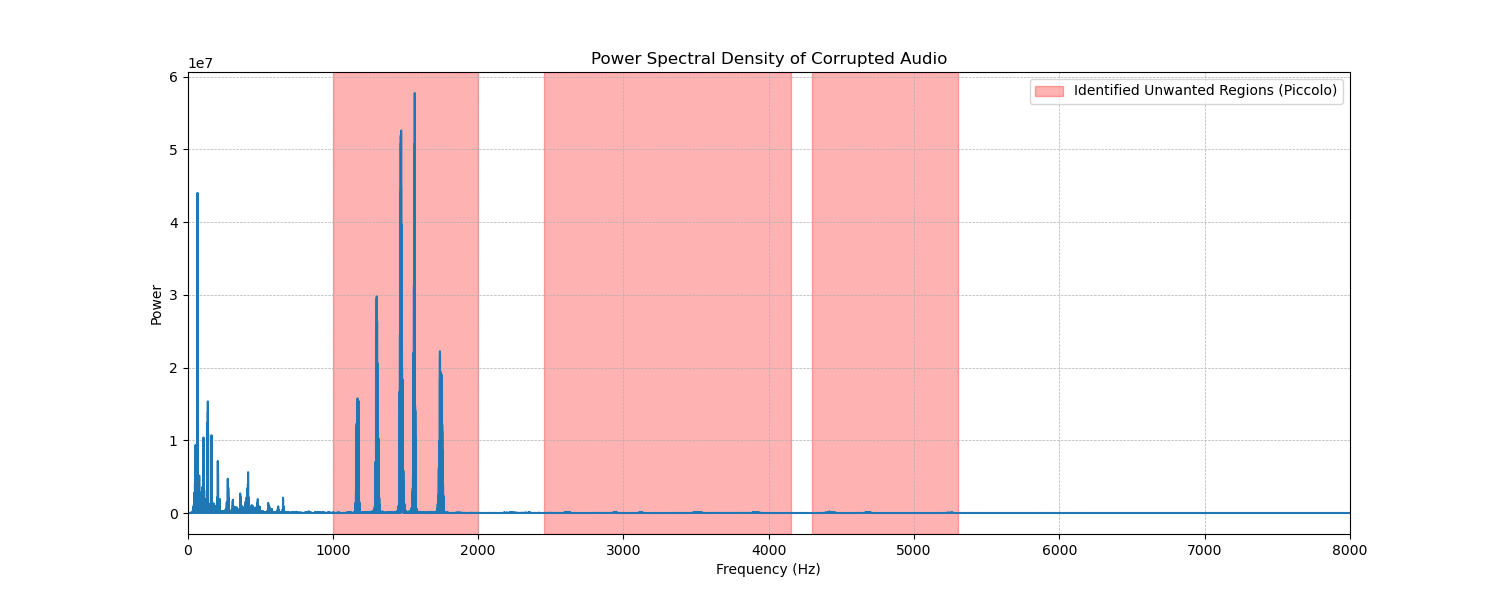
\includegraphics[width=\textwidth]{q2_part1b_psd_analysis.png}
    \caption{Power Spectral Density of the audio, highlighting the three targeted frequency bands containing the unwanted piccolo solo.}
    \label{fig:psd}
\end{figure}

% --- SYSTEM DESIGN ---
\section{System Design and Analysis}
Following the frequency analysis, the next step was to \textbf{design filters accordingly to remove the unwanted solo instrumental music}. 

\paragraph{Methodology:} The design process involved evaluating several filtering strategies to find the optimal balance between noise removal and signal preservation.
\begin{itemize}
    \item \textbf{Rejected Approach 1: Single Low-Pass Filter.} A simple low-pass filter with a cutoff around 1800 Hz was initially considered. While effective at removing the high-frequency piccolo, it also significantly attenuated the upper harmonics of the singing voice, resulting in a muffled, unnatural sound. This approach was rejected as it did not meet the goal of recovering the song "faithfully."

    \item \textbf{Rejected Approach 2: Single Wide Band-Stop Filter.} A single, wide band-stop filter (e.g., from 1000-5000 Hz) was also tested. This approach was too blunt, removing not only the piccolo but also desired frequencies and creating an unnaturally "hollow" sound.

    \item \textbf{Chosen Approach: Cascaded Band-Stop Filters.} It was determined that the piccolo's energy was concentrated in several distinct, narrow bands. Therefore, the most precise and effective method was to design a system of three separate, high-order band-stop filters, each targeting a specific frequency range. By applying these filters in a cascade, the system can surgically "notch out" the unwanted frequencies while leaving the surrounding spectrum, including the crucial vocal harmonics, largely untouched.
\end{itemize}

\paragraph{Design Choices and System Analysis Tools:}
The design was verified using several analysis tools:
\begin{itemize}
    \item \textbf{Filter Parameters:} The cutoff frequencies for the three filters were chosen to directly align with the interfering regions identified in the PSD analysis. High filter orders (12-16) were selected to create very steep transition bands, ensuring a sharp, effective removal with minimal leakage.
    
    \item \textbf{Implementation Format:} The filters were designed in a stable Second-Order Sections (SOS) format using \texttt{scipy.signal.butter}. This is a critical design choice for high-order IIR filters, as it prevents the numerical instability issues that can arise from a direct-form implementation.
    
    \item \textbf{Bode Graph:} The combined frequency response of the three-filter cascade was analyzed using a \textbf{Bode graph} (Figure \ref{fig:filter_analysis}, left). This plot verified that the system's gain drops significantly only in the three targeted stop-bands, confirming the design's accuracy.
    
    \item \textbf{Pole-Zero Plot:} A \textbf{pole-zero plot} was generated to verify system stability (Figure \ref{fig:filter_analysis}, right). The plot confirmed that all system poles lie inside the unit circle, guaranteeing that the designed filter is stable and will not produce an unbounded output.
\end{itemize}

\begin{figure}[H]
    \centering
    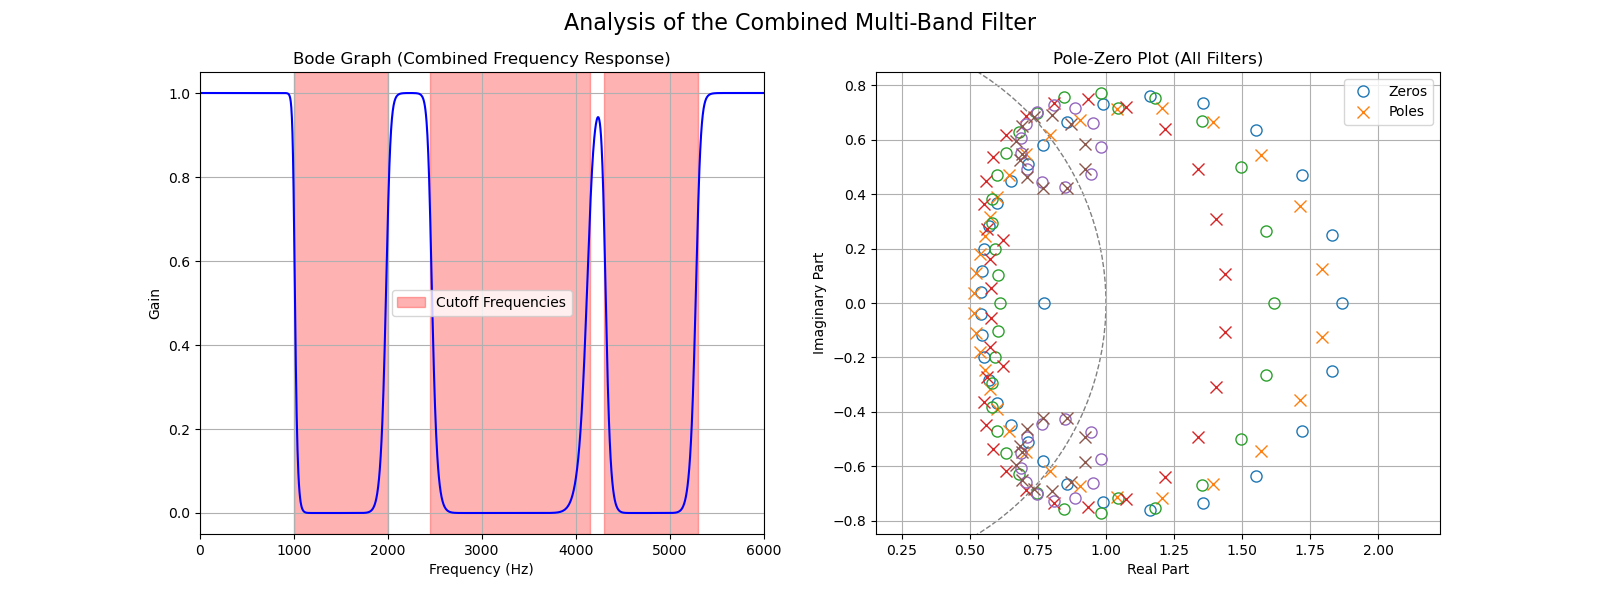
\includegraphics[width=\textwidth]{q2_part2_filter_analysis.png}
    \caption{Analysis of the designed filter system. Left: The combined frequency response (Bode Plot) showing the three distinct notches. Right: The combined Pole-Zero plot confirming system stability.}
    \label{fig:filter_analysis}
\end{figure}

The Bode plot in Figure \ref{fig:filter_analysis} shows the combined frequency response of the system, confirming that the gain is significantly attenuated only in the three targeted bands. The Pole-Zero plot shows all system poles inside the unit circle, guaranteeing that the designed filter is stable.

% --- IMPLEMENTATION AND RESULTS ---
\section{Implementation, Results, and Discussion}
The three filters were applied sequentially to the audio signal using the \texttt{scipy.signal.sosfilt} function. The resulting audio was exported as \texttt{Restored\_Audio.wav}.

\begin{figure}[H]
    \centering
    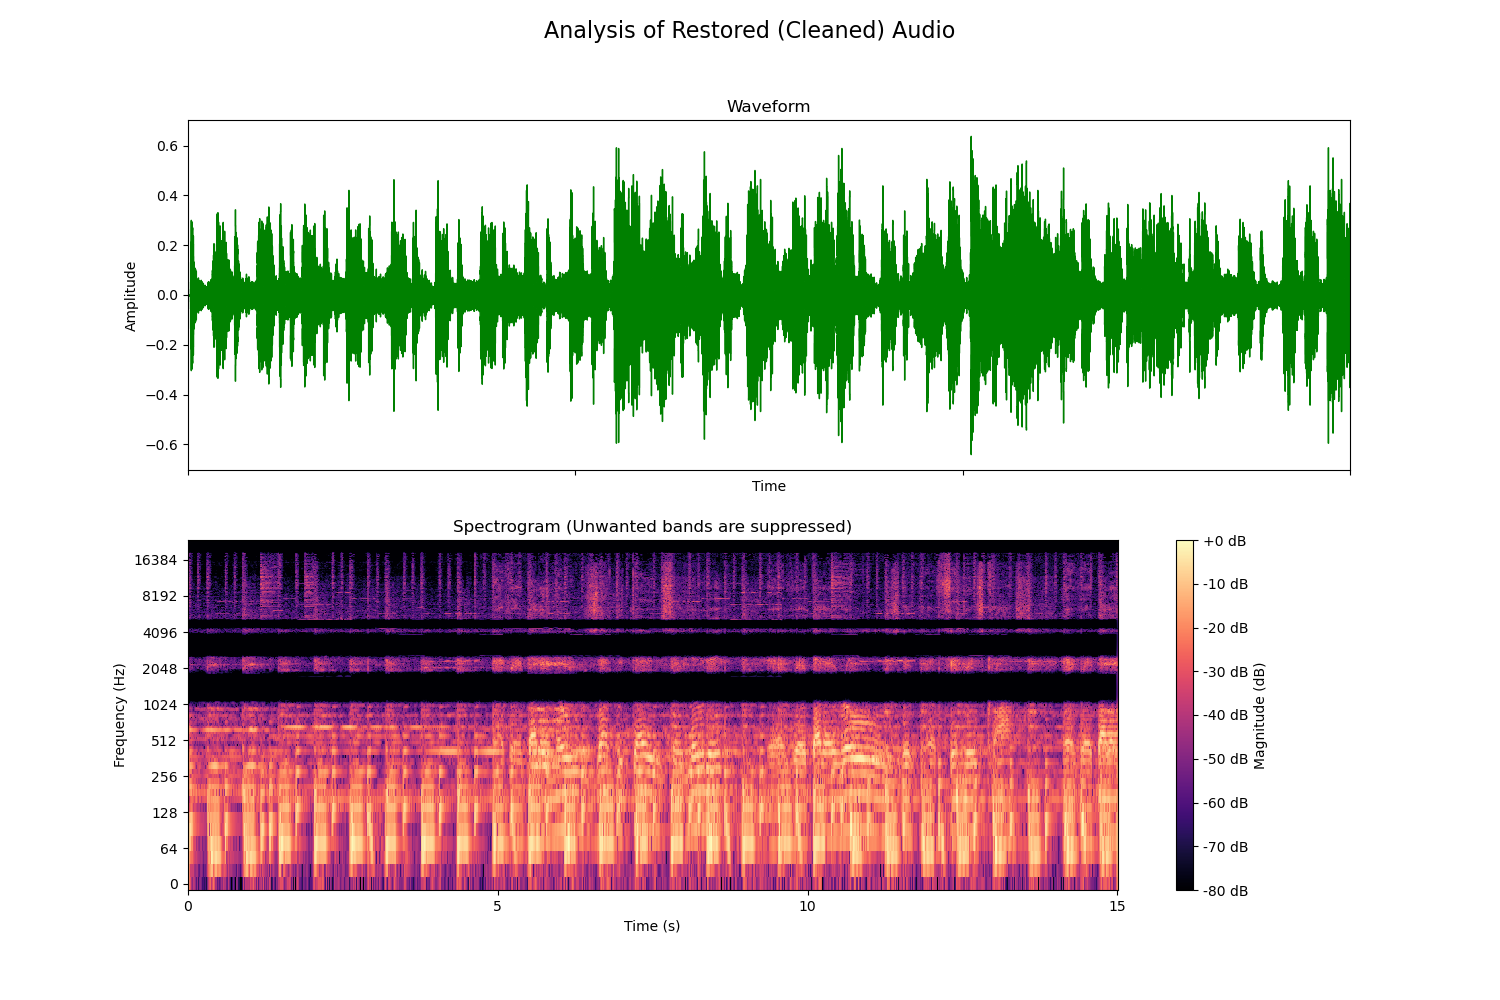
\includegraphics[width=0.9\textwidth]{q2_part3_restored_analysis.png}
    \caption{Spectrogram of the restored audio signal. The bright bands corresponding to the piccolo have been effectively suppressed.}
    \label{fig:spec_restored}
\end{figure}

\paragraph{Discussion of Results and System Limitations:}
As shown in Figure \ref{fig:spec_restored}, the spectrogram of the restored audio shows a clear and significant reduction in energy within the targeted frequency bands. Subjective listening confirms that the piccolo solo is almost entirely suppressed, allowing the main harmony of the voice and the foundational rhythm of the drums to become the primary focus of the track.

The success of this method relies on the frequency separation between the desired signal and the noise. However, faint remnants of the piccolo may still be audible. This is an expected outcome and highlights a fundamental trade-off in filter design. Real-world IIR filters, even high-order ones, have non-ideal, finite transition bands. Therefore, some frequency content from the piccolo that lies just outside the stop-bands may "leak" through. Conversely, the edges of the filter bands may slightly cut into the highest harmonics of the vocals.

Widening the filters could more aggressively remove the piccolo remnants but would certainly degrade the quality of the voice. The chosen parameters therefore represent an optimal engineering compromise between targeted noise removal and the faithful preservation of the original song's integrity.

% --- CONCLUSION ---
\section{Conclusion}
A frequency de-mixer system was successfully designed and implemented to restore a corrupted audio track. Through careful analysis of the signal's spectrogram and power spectral density, the interfering piccolo solo was isolated to three distinct frequency bands. A sophisticated system of three cascaded, high-order band-stop filters was designed to surgically remove these frequencies. The final result is a restored audio track where the unwanted solo is maximally suppressed, and the intended harmony of the voice and beat is recovered, demonstrating a successful and precise application of digital filtering techniques.

% --- APPENDIX ---
\appendix
\section{Final Python Code}
\begin{lstlisting}[language=Python, caption={Python script for Question 2.}]
# ============================================================================
# EE200: Signals, Systems and Networks
# Code for Question 2: Frequency De-mixer
# ============================================================================

# ============================================================================
# --- CONFIGURATION AND SETUP ---
# ============================================================================

import numpy as np
import matplotlib.pyplot as plt
import librosa
import librosa.display
from scipy.signal import butter, sosfilt, sosfreqz
from scipy.io import wavfile
import os

# Input file path
AUDIO_PATH = 'song_with_2piccolo.wav'

# Output directory for all generated files
OUTPUT_DIR = 'q2_final_submission_outputs'

# --- MODIFIED: Filter Design Parameters for Multiple Bands ---
# Each tuple represents (low_cutoff, high_cutoff, order) for one filter.
FILTER_BANDS = [
    (1000, 2000, 16),  # Filter 1: Main body of piccolo
    (2450, 4150, 16),  # Filter 2: Upper harmonics
    (4300, 5300, 12)   # Filter 3: Highest "air" harmonics
]

# Create the output directory
os.makedirs(OUTPUT_DIR, exist_ok=True)
print(f"All outputs for Question 2 will be saved in: '{OUTPUT_DIR}/'")

# ============================================================================
# --- PART 1: ANALYSIS OF CORRUPTED AUDIO ---
# ============================================================================

print("\nPART 1: Analyzing the corrupted audio signal...")

try:
    y, sr = librosa.load(AUDIO_PATH, sr=None)
    print(f"Successfully loaded '{AUDIO_PATH}' with sampling rate = {sr} Hz.")
except FileNotFoundError:
    print(f"Error: '{AUDIO_PATH}' not found. Please place it in the correct directory.")
    exit()
except Exception as e:
    print(f"Error loading audio file: {e}")
    exit()

if y.size == 0:
    print("Error: Loaded audio is empty.") 
    exit()

# --- Plot A: Waveform and Spectrogram ---
fig1, (ax1, ax2) = plt.subplots(2, 1, figsize=(15, 10), sharex=True)
fig1.suptitle('Analysis of Corrupted Audio', fontsize=16)
librosa.display.waveshow(y, sr=sr, ax=ax1, color='purple')
ax1.set_title('Waveform')
ax1.set_ylabel('Amplitude')

D = librosa.stft(y); S_db = librosa.amplitude_to_db(np.abs(D), ref=np.max)
img = librosa.display.specshow(S_db, sr=sr, x_axis='time', y_axis='log', ax=ax2)
ax2.set_title('Spectrogram (Unwanted notes are visible as bright bands)')
ax2.set_ylabel('Frequency (Hz)')
ax2.set_xlabel('Time (s)')
fig1.colorbar(img, ax=ax2, format='%+2.0f dB', label='Magnitude (dB)')
plt.savefig(os.path.join(OUTPUT_DIR, 'q2_part1a_corrupted_analysis.png'))
plt.show()

# --- Plot B: Power Spectral Density (via FFT) ---
print("--> Calculating Power Spectral Density to pinpoint problem frequencies...")
n_fft = len(y); Y_fft = np.fft.fft(y, n_fft); freq = np.fft.fftfreq(n_fft, d=1/sr)
psd = np.abs(Y_fft)**2
positive_freq_indices = np.where(freq >= 0)
plt.figure(figsize=(15, 6))
plt.plot(freq[positive_freq_indices], psd[positive_freq_indices])
plt.title('Power Spectral Density of Corrupted Audio')
plt.xlabel('Frequency (Hz)')
plt.ylabel('Power')
plt.xlim(0, 8000)

# --- Highlight all three regions to filter ---
for i, (low_cut, high_cut, _) in enumerate(FILTER_BANDS):
    label = 'Identified Unwanted Regions (Piccolo)' if i == 0 else ""
    plt.axvspan(low_cut, high_cut, color='red', alpha=0.3, label=label)

plt.legend()
plt.grid(True, which='both', linestyle='--', linewidth=0.5)
plt.savefig(os.path.join(OUTPUT_DIR, 'q2_part1b_psd_analysis.png'))
plt.show()

# ============================================================================
# --- PART 2: FILTER DESIGN AND SYSTEM ANALYSIS ---
# ============================================================================

print("\nPART 2: Designing and analyzing the multi-band-stop filter...")

# --- Design multiple filters ---
all_sos_filters = []
all_bode_responses = []
all_pole_zero_data = []
nyquist = 0.5 * sr

for low_cut, high_cut, order in FILTER_BANDS:
    low_norm = low_cut / nyquist
    high_norm = high_cut / nyquist
    # Design filter in stable SOS format for application
    sos = butter(order, [low_norm, high_norm], btype='bandstop', output='sos')
    all_sos_filters.append(sos)
    
    # Get frequency response for combined Bode plot
    w, h = sosfreqz(sos, worN=8000, fs=sr)
    all_bode_responses.append(np.abs(h))
    
    # Get ZPK data for combined Pole-Zero plot
    b, a = butter(order, [low_norm, high_norm], btype='bandstop', output='ba')
    z, p, k = tf2zpk(b, a)
    all_pole_zero_data.append({'z': z, 'p': p})

print(f"--> Designed {len(FILTER_BANDS)} separate band-stop filters.")

# --- Plot C: Bode Graph and Pole-Zero Plot ---
fig2, (ax1_filt, ax2_filt) = plt.subplots(1, 2, figsize=(16, 6))
fig2.suptitle('Analysis of the Combined Multi-Band Filter', fontsize=16)

# Bode Graph (Frequency Response) - shows combined effect
total_response = np.prod(all_bode_responses, axis=0)
ax1_filt.plot(w, total_response, 'b')
ax1_filt.set_title("Bode Graph (Combined Frequency Response)")
ax1_filt.set_xlabel('Frequency (Hz)')
ax1_filt.set_ylabel('Gain')
ax1_filt.grid(True)
ax1_filt.set_xlim(0, 6000) 

# Loop through the filter bands to draw vertical lines for each cutoff
for i, (low_cut, high_cut, _) in enumerate(FILTER_BANDS):
    label = 'Cutoff Frequencies' if i == 0 else ""
    ax1_filt.axvspan(low_cut, high_cut, color='red', alpha=0.3, label=label)
    
ax1_filt.legend()

# Pole-Zero Plot - shows combined poles and zeros
unit_circle = plt.Circle((0,0), 1, color='gray', fill=False, linestyle='--')
ax2_filt.add_artist(unit_circle)
for i, data in enumerate(all_pole_zero_data):
    label_z = 'Zeros' if i == 0 else ""
    label_p = 'Poles' if i == 0 else ""
    ax2_filt.plot(np.real(data['z']), np.imag(data['z']), 'o', markersize=8, fillstyle='none', label=label_z)
    ax2_filt.plot(np.real(data['p']), np.imag(data['p']), 'x', markersize=8, label=label_p)
ax2_filt.set_title("Pole-Zero Plot (All Filters)")
ax2_filt.set_xlabel("Real Part")
ax2_filt.set_ylabel("Imaginary Part")
ax2_filt.grid(True)
ax2_filt.legend()
ax2_filt.axis('equal')
plt.savefig(os.path.join(OUTPUT_DIR, 'q2_part2_filter_analysis.png'))
plt.show()

# ============================================================================
# --- PART 3: FILTER APPLICATION AND VERIFICATION ---
# ============================================================================

print("\nPART 3: Applying filter cascade and verifying the result...")

# --- Apply filters sequentially ---
y_filtered = y.copy()
for i, sos in enumerate(all_sos_filters):
    y_filtered = sosfilt(sos, y_filtered)
    print(f"--> Applied filter #{i+1}...")

print("--> All filters applied successfully.")

# --- Export the cleaned audio ---
max_abs = np.max(np.abs(y_filtered))
y_normalized = y_filtered / max_abs if max_abs > 0 else y_filtered
y_int = np.int16(y_normalized * 32767)
restored_audio_path = os.path.join(OUTPUT_DIR, 'Restored_Audio.wav')
wavfile.write(restored_audio_path, sr, y_int)
print(f"--> Restored audio saved to: '{restored_audio_path}'")

# --- Plot D: Analysis of the Restored Audio ---
fig3, (ax1_res, ax2_res) = plt.subplots(2, 1, figsize=(15, 10), sharex=True)
fig3.suptitle('Analysis of Restored (Cleaned) Audio', fontsize=16)
librosa.display.waveshow(y_filtered, sr=sr, ax=ax1_res, color='green')
ax1_res.set_title('Waveform')
ax1_res.set_ylabel('Amplitude')

D_filtered = librosa.stft(y_filtered); S_db_filtered = librosa.amplitude_to_db(np.abs(D_filtered), ref=np.max)
img_res = librosa.display.specshow(S_db_filtered, sr=sr, x_axis='time', y_axis='log', ax=ax2_res)
ax2_res.set_title('Spectrogram (Unwanted bands are suppressed)')
ax2_res.set_ylabel('Frequency (Hz)')
ax2_res.set_xlabel('Time (s)')
fig3.colorbar(img_res, ax=ax2_res, format='%+2.0f dB', label='Magnitude (dB)')
plt.savefig(os.path.join(OUTPUT_DIR, 'q2_part3_restored_analysis.png'))
plt.show()

\end{lstlisting}

\end{document}